\documentclass[12pt,letterpaper]{article}
\usepackage{graphicx,textcomp}
\usepackage{natbib}
\usepackage{setspace}
\usepackage{fullpage}
\usepackage{color}
\usepackage[reqno]{amsmath}
\usepackage{amsthm}
\usepackage{fancyvrb}
\usepackage{amssymb,enumerate}
\usepackage[all]{xy}
\usepackage{endnotes}
\usepackage{lscape}
\newtheorem{com}{Comment}
\usepackage{float}
\usepackage{hyperref}
\newtheorem{lem} {Lemma}
\newtheorem{prop}{Proposition}
\newtheorem{thm}{Theorem}
\newtheorem{defn}{Definition}
\newtheorem{cor}{Corollary}
\newtheorem{obs}{Observation}
\usepackage[compact]{titlesec}
\usepackage{dcolumn}
\usepackage{tikz}
\usetikzlibrary{arrows}
\usepackage{multirow}
\usepackage{xcolor}
\newcolumntype{.}{D{.}{.}{-1}}
\newcolumntype{d}[1]{D{.}{.}{#1}}
\definecolor{light-gray}{gray}{0.65}
\usepackage{url}
\usepackage{listings}
\usepackage{color}

\definecolor{codegreen}{rgb}{0,0.6,0}
\definecolor{codegray}{rgb}{0.5,0.5,0.5}
\definecolor{codepurple}{rgb}{0.58,0,0.82}
\definecolor{backcolour}{rgb}{0.95,0.95,0.92}

\lstdefinestyle{mystyle}{
	backgroundcolor=\color{backcolour},   
	commentstyle=\color{codegreen},
	keywordstyle=\color{magenta},
	numberstyle=\tiny\color{codegray},
	stringstyle=\color{codepurple},
	basicstyle=\footnotesize,
	breakatwhitespace=false,         
	breaklines=true,                 
	captionpos=b,                    
	keepspaces=true,                 
	numbers=left,                    
	numbersep=5pt,                  
	showspaces=false,                
	showstringspaces=false,
	showtabs=false,                  
	tabsize=2
}
\lstset{style=mystyle}
\newcommand{\Sref}[1]{Section~\ref{#1}}
\newtheorem{hyp}{Hypothesis}

\title{Problem Set 1}
\date{Due: January 29, 2020}
\author{QTM 200: Applied Regression Analysis}

\begin{document}
%\lstinputlisting{/Users/chloesutter/GitHub/QTM200Spring2020/problem_sets/PS1/Sutter_ProblemSet1.R}



\title{Problem Set 1}
\date{Due: January 27, 2020}
\author{QTM 200: Applied Regression Analysis, Chloe Sutter}


\section*{Question 1 (25 points)}
A private school counselor was curious about the average of IQ of the students in her school and took a random sample of 25 students' IQ scores. The following is the data set:
\lstinputlisting[language=R, firstline=47, lastline=47]{Sutter_ProblemSet1.R}  
\vspace{.5cm}
\noindent Find a 90\% confidence interval for the student IQ in the school assuming the population of IQ from which our random sample has been selected is normally distributed. 
\vspace{.5cm} 
\lstinputlisting[language=R, firstline=51, lastline=59]{Sutter_ProblemSet1.R}
\noindent A 90 Percent Confidence Interval = (91.65, 105.22)
\vspace{1cm}

\section*{Question 2 (25 points)}
\noindent A private school counselor was curious  whether  the average of IQ of the students in her school is higher than the average IQ score 100 among all the schools in the country. \noindent She took a random sample of 25 students' IQ scores. The following is the data set:
\lstinputlisting[language=R, firstline=46, lastline=46]{PS1.R}
\vspace{.5cm}
\lstinputlisting[language=R, firstline=70, lastline=70] {Sutter_ProblemSet1.R}
\noindent Conduct a test with 0.05 significance level assuming the population of IQ from which our random sample has been selected is normally distributed. 
\vspace{.5cm}
\lstinputlisting[language=R, firstline=70, lastline=70] {Sutter_ProblemSet1.R}
\noindent data fits the assumptions of random sampling, quantitative data, and normal distribution.
\noindent state hypotheses: H0 = 100 , HA does not = 100
\noindent calculate the test statistic:
\lstinputlisting[language=R, firstline=78, lastline=78] {Sutter_ProblemSet1.R}
\lstinputlisting[language=R, firstline=80, lastline=83] {Sutter_ProblemSet1.R}
\noindent find P value:
\lstinputlisting[language=R, firstline=86, lastline=86] {Sutter_ProblemSet1.R}
\noindent P value = 0.56. Since p < α, we conclude that the evidence supports the null hypothesis. The average IQ of the students in her school is not higher than the average IQ score \noindent 100 among all the schools in the country.

\vspace{1cm}
	\section*{Question 3 (50 points)}

\vspace{.5cm}
\lstinputlisting[language=R, firstline=103, lastline=104]{Sutter_ProblemSet1.R}  
\vspace{.5cm}
\noindent Researchers are curious about what affects the education expenditure on public education. The following is availabe variables in a data set about the education expenditure. \\
\vspace{.5cm}




\begin{tabular}{r|l}
	\texttt{State} &\emph{50 states in US} \\
	\texttt{Y} & \emph{per capita expenditure on public education}\\
	\texttt{X1} &\emph{per capita personal income} \\
	\texttt{X2} &  \emph{Number of residents per thousand under 18 years of age}\\
	\texttt{X3} &  \emph{Number of people per thousand residing in urban areas} \\
	\texttt{Region} &  \emph{1=Northeast, 2= North Central, 3= South, 4=West} \\

\end{tabular}

\vspace{1cm}
\begin{itemize}

\item

Please plot the relationships among \emph{Y}, \emph{X1}, \emph{X2}, and \emph{X3}? What are the correlations among them? Describe the graph and the relationships among them.
\vspace{.5cm}

\noindent Plot Y
\lstinputlisting[language=R, firstline=109, lastline=109]{Sutter_ProblemSet1.R}  
\begin{figure}
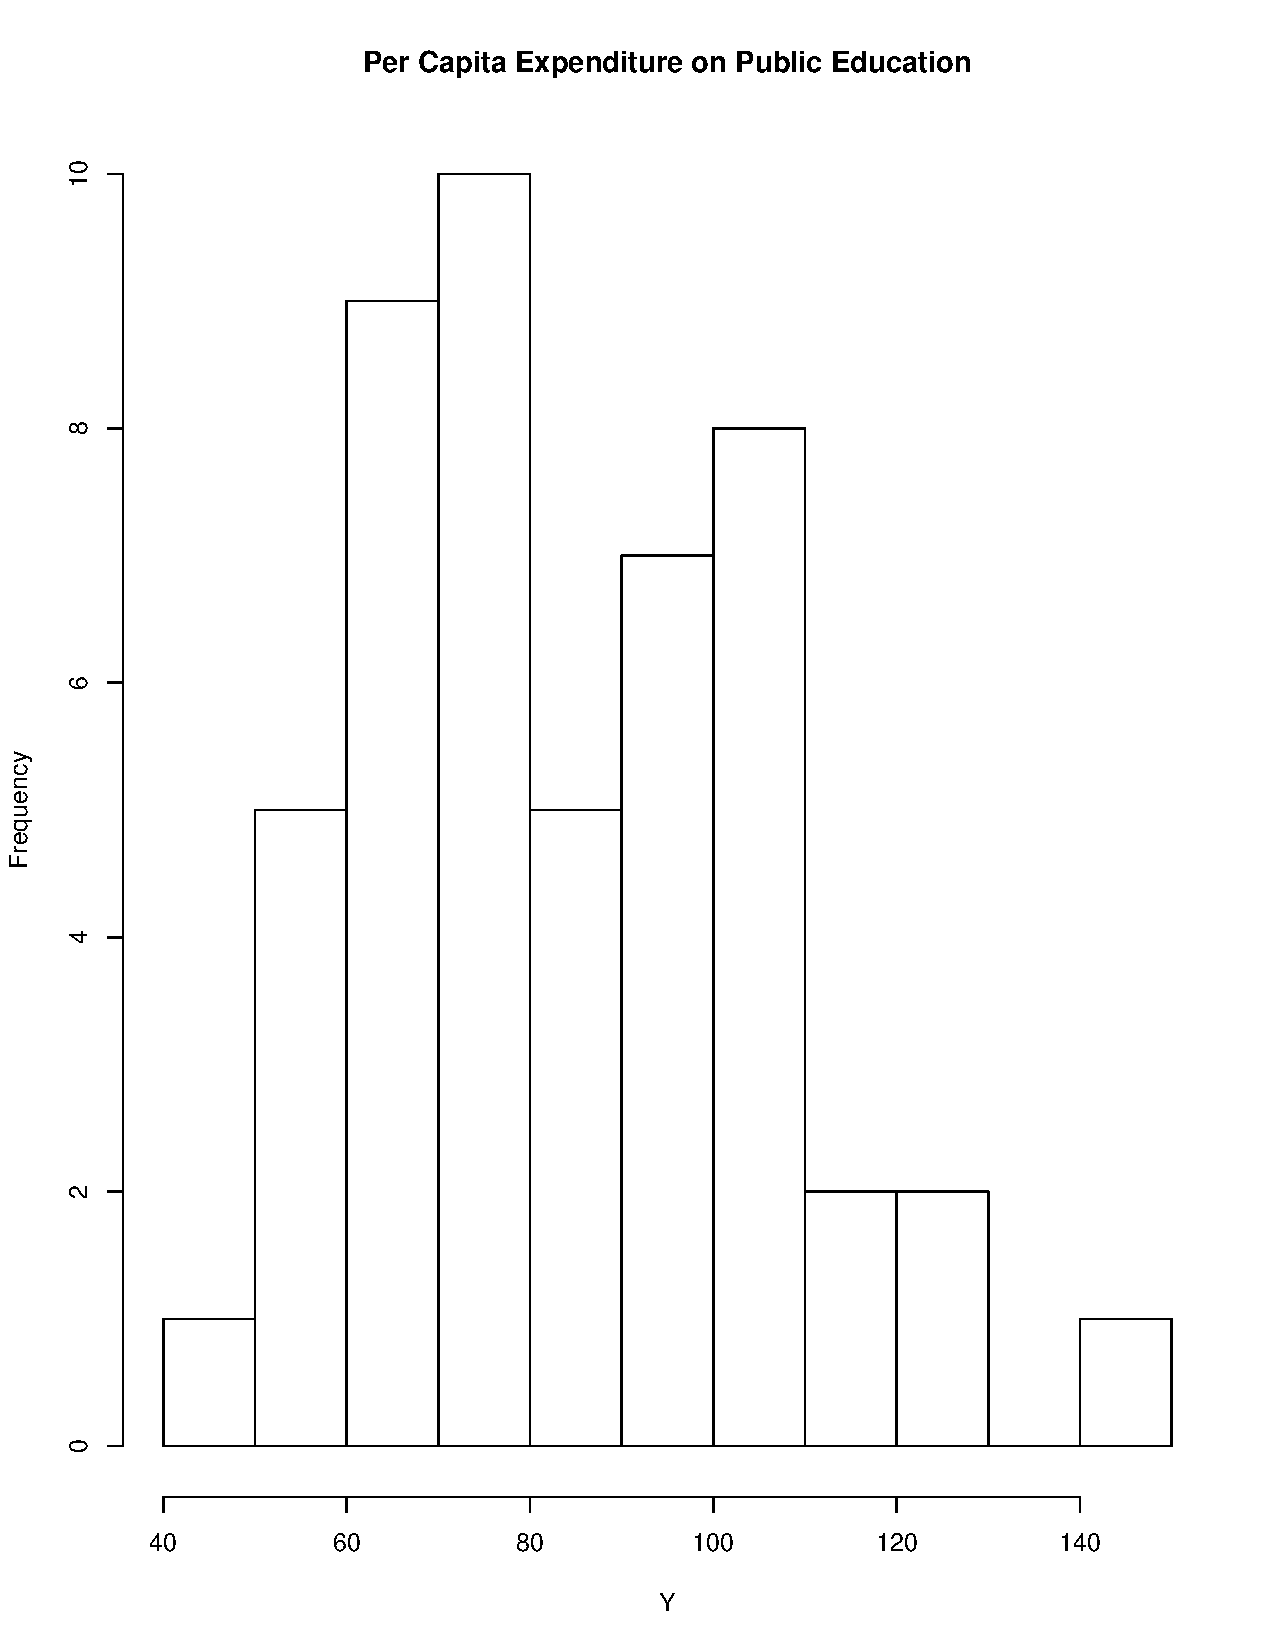
\includegraphics[width=50mm,scale=0.5]{Y.pdf}
\end{figure} 
\noindent The data for Y presents a bimodal histogram, with two spikes. The first at around 60 and the second at 100. 
\vspace{.5cm}

\noindent Plot X1
\lstinputlisting[language=R, firstline=115, lastline=115]{Sutter_ProblemSet1.R}
\begin{figure}
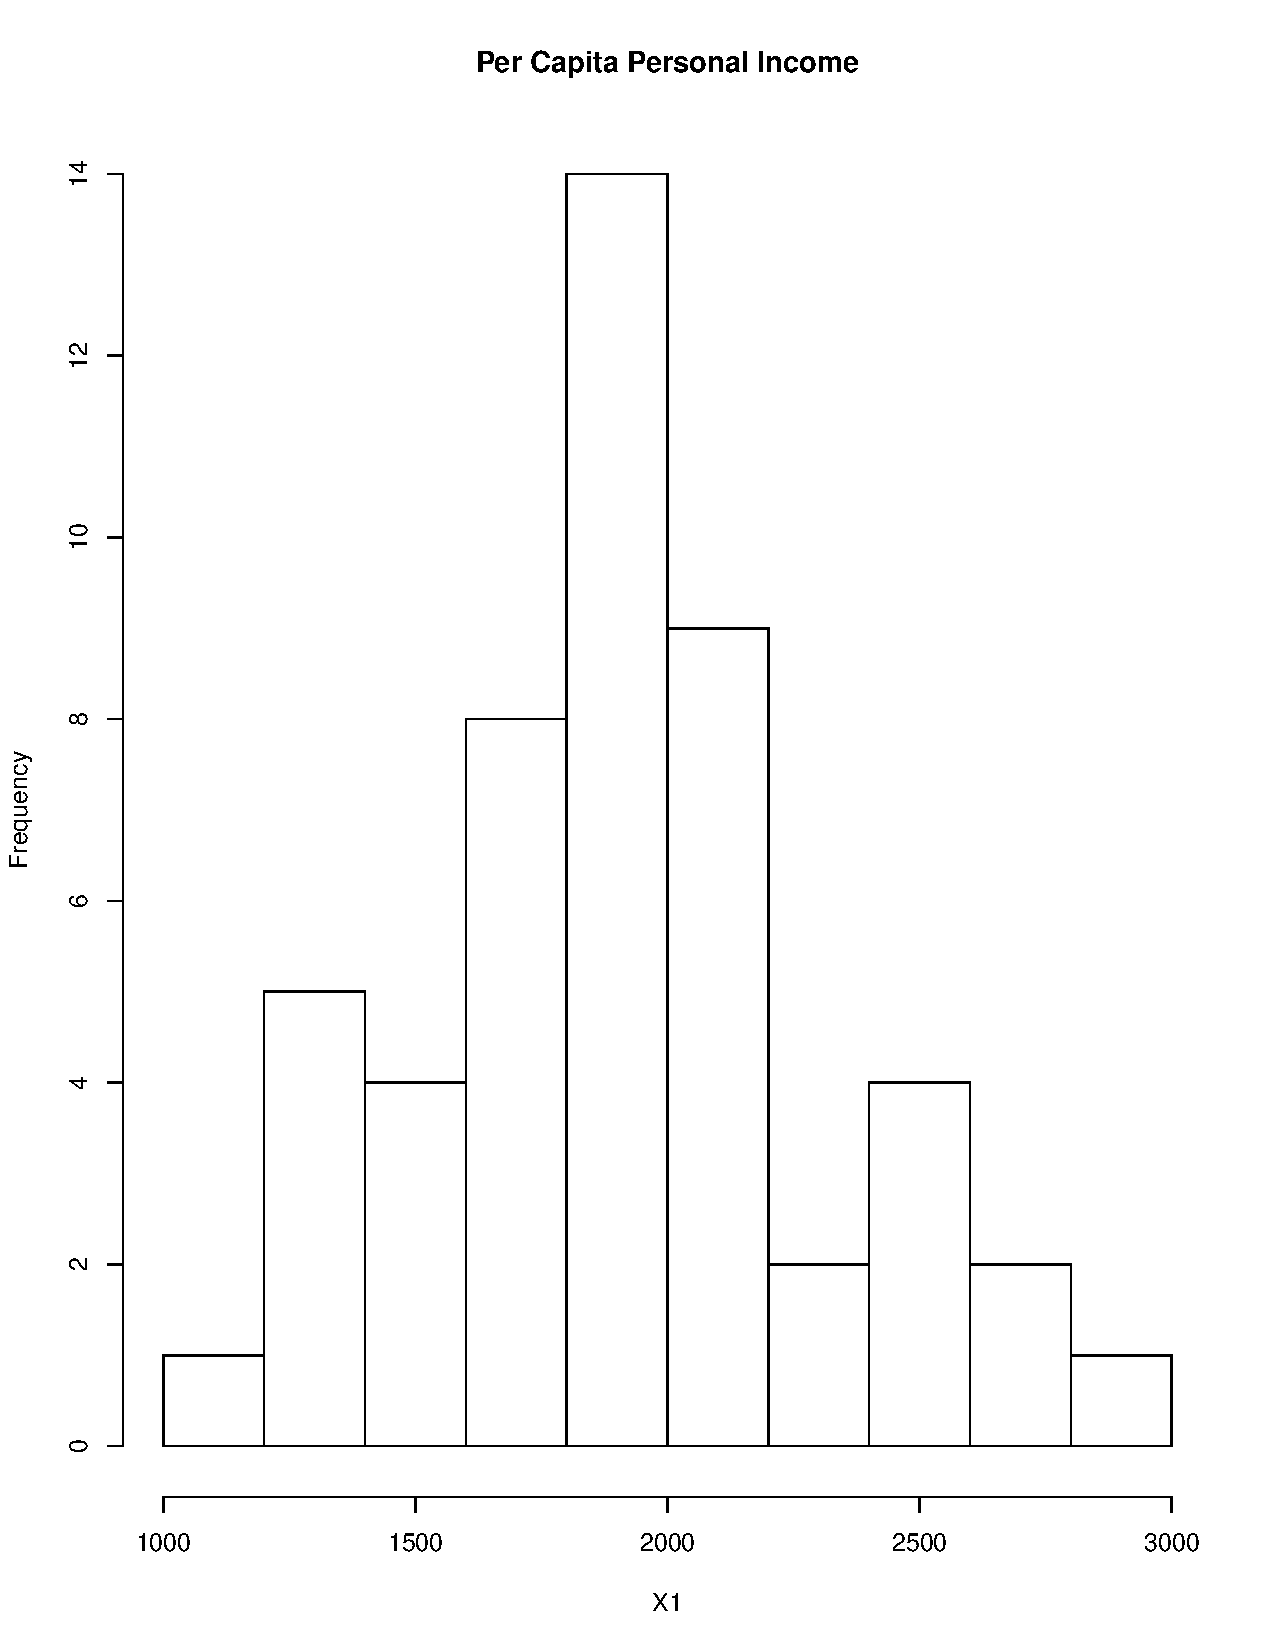
\includegraphics[width=50mm,scale=0.5]{X1.pdf}
\end{figure} 
\noindent X1 displays a relatively normal distribution, with its peak per capita personal income at about 2000. 

 
\vspace{.5cm}
\noindent Plot X2
\lstinputlisting[language=R, firstline=119, lastline=119]{Sutter_ProblemSet1.R}
\begin{figure}
\includegraphics[width=50mm,scale=0.5]={X2.pdf}
\end{figure} 
\noindent X2 has the highest frequency at about 400, with a largely right-skewed distribution. Thus, there is a higher frequency of residents per thousand under 18 between the values of 300 and 400.

\vspace{.5cm}
\noindent Plot X3
\lstinputlisting[language=R, firstline=123, lastline=123]{Sutter_ProblemSet1.R}
\begin{figure}
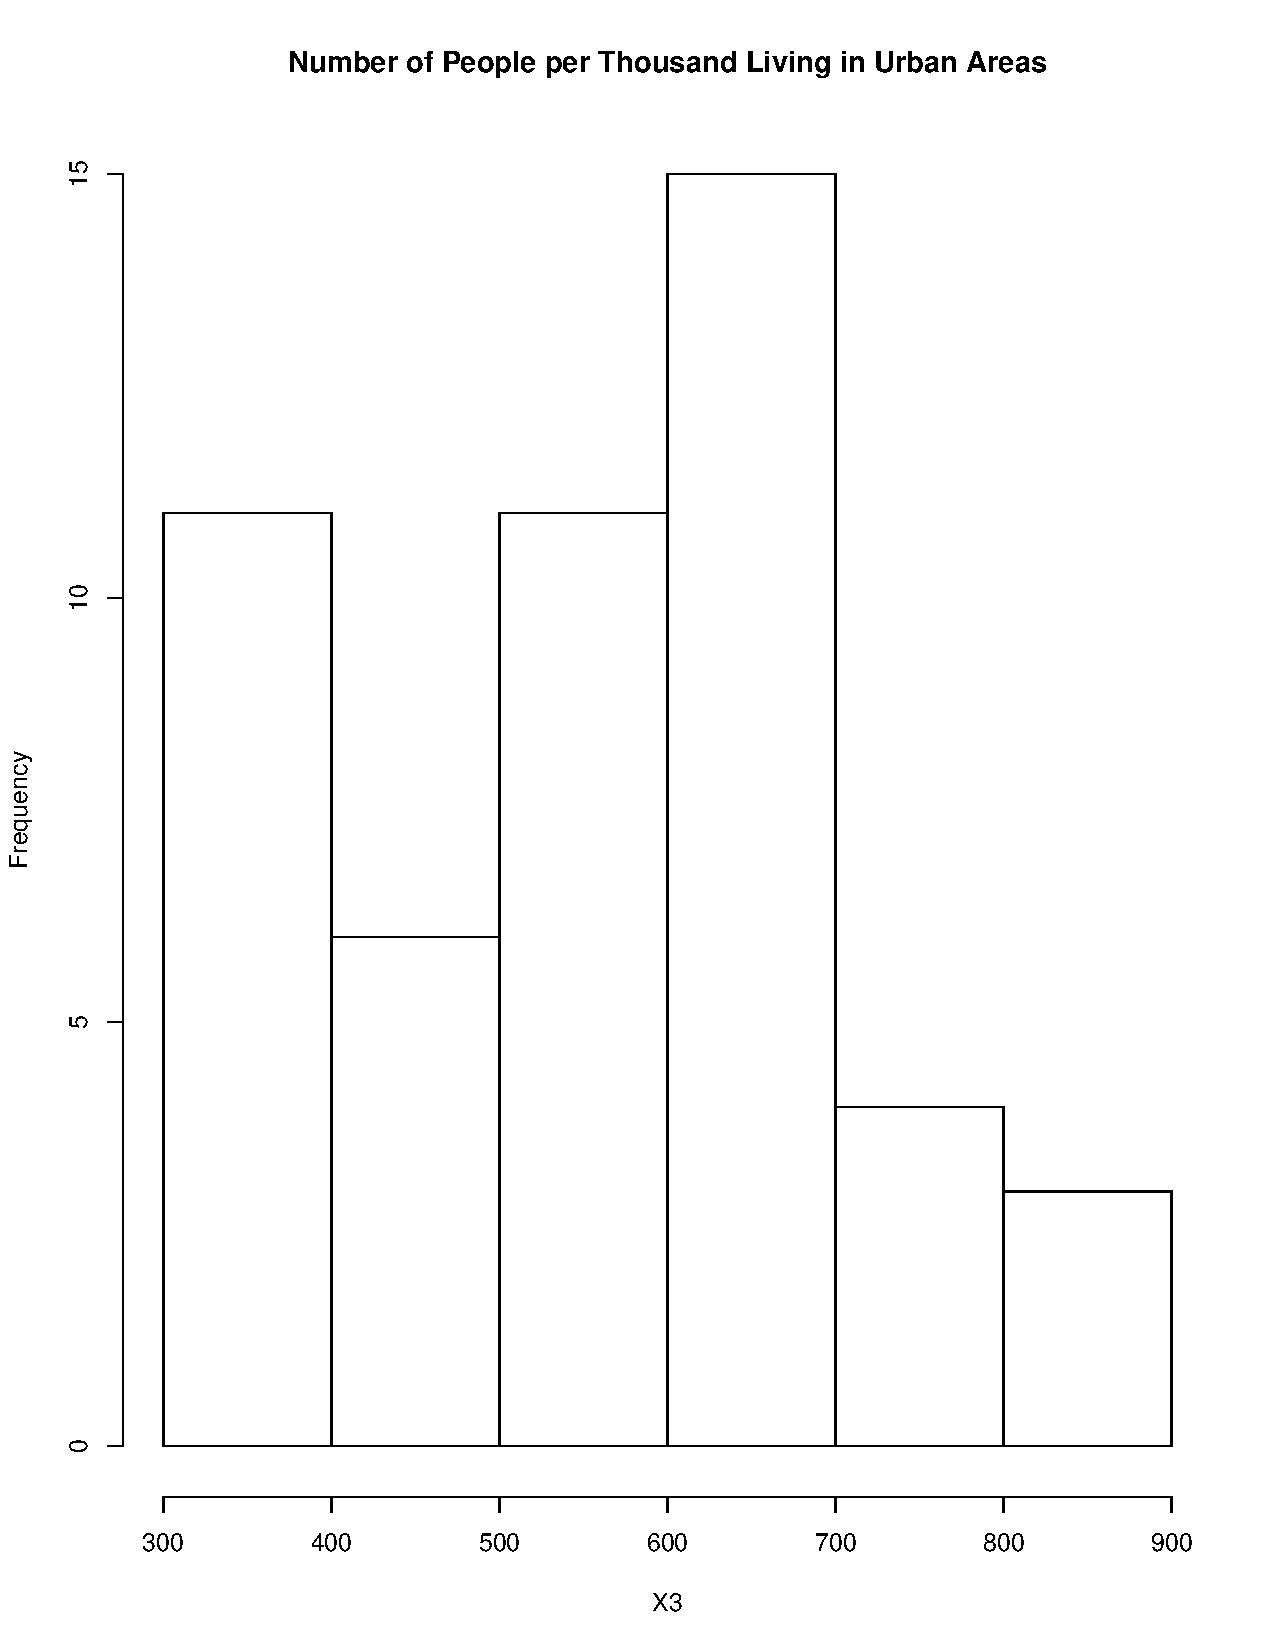
\includegraphics[width=50mm,scale=0.5]{X3.pdf}
\end{figure} 
\noindent X3 has the highest frequency at its mean, which is around 600. It is slightly skewed right, less significantly than X2.
\vspace{1cm}

\item
Please plot the relationship between \emph{Y} and \emph{Region}? On average, which region does have the highest per capita expenditure on public education?
\vspace{.5cm}
\lstinputlisting[language=R, firstline=127, lastline=127]{Sutter_ProblemSet1.R}
\begin{figure}
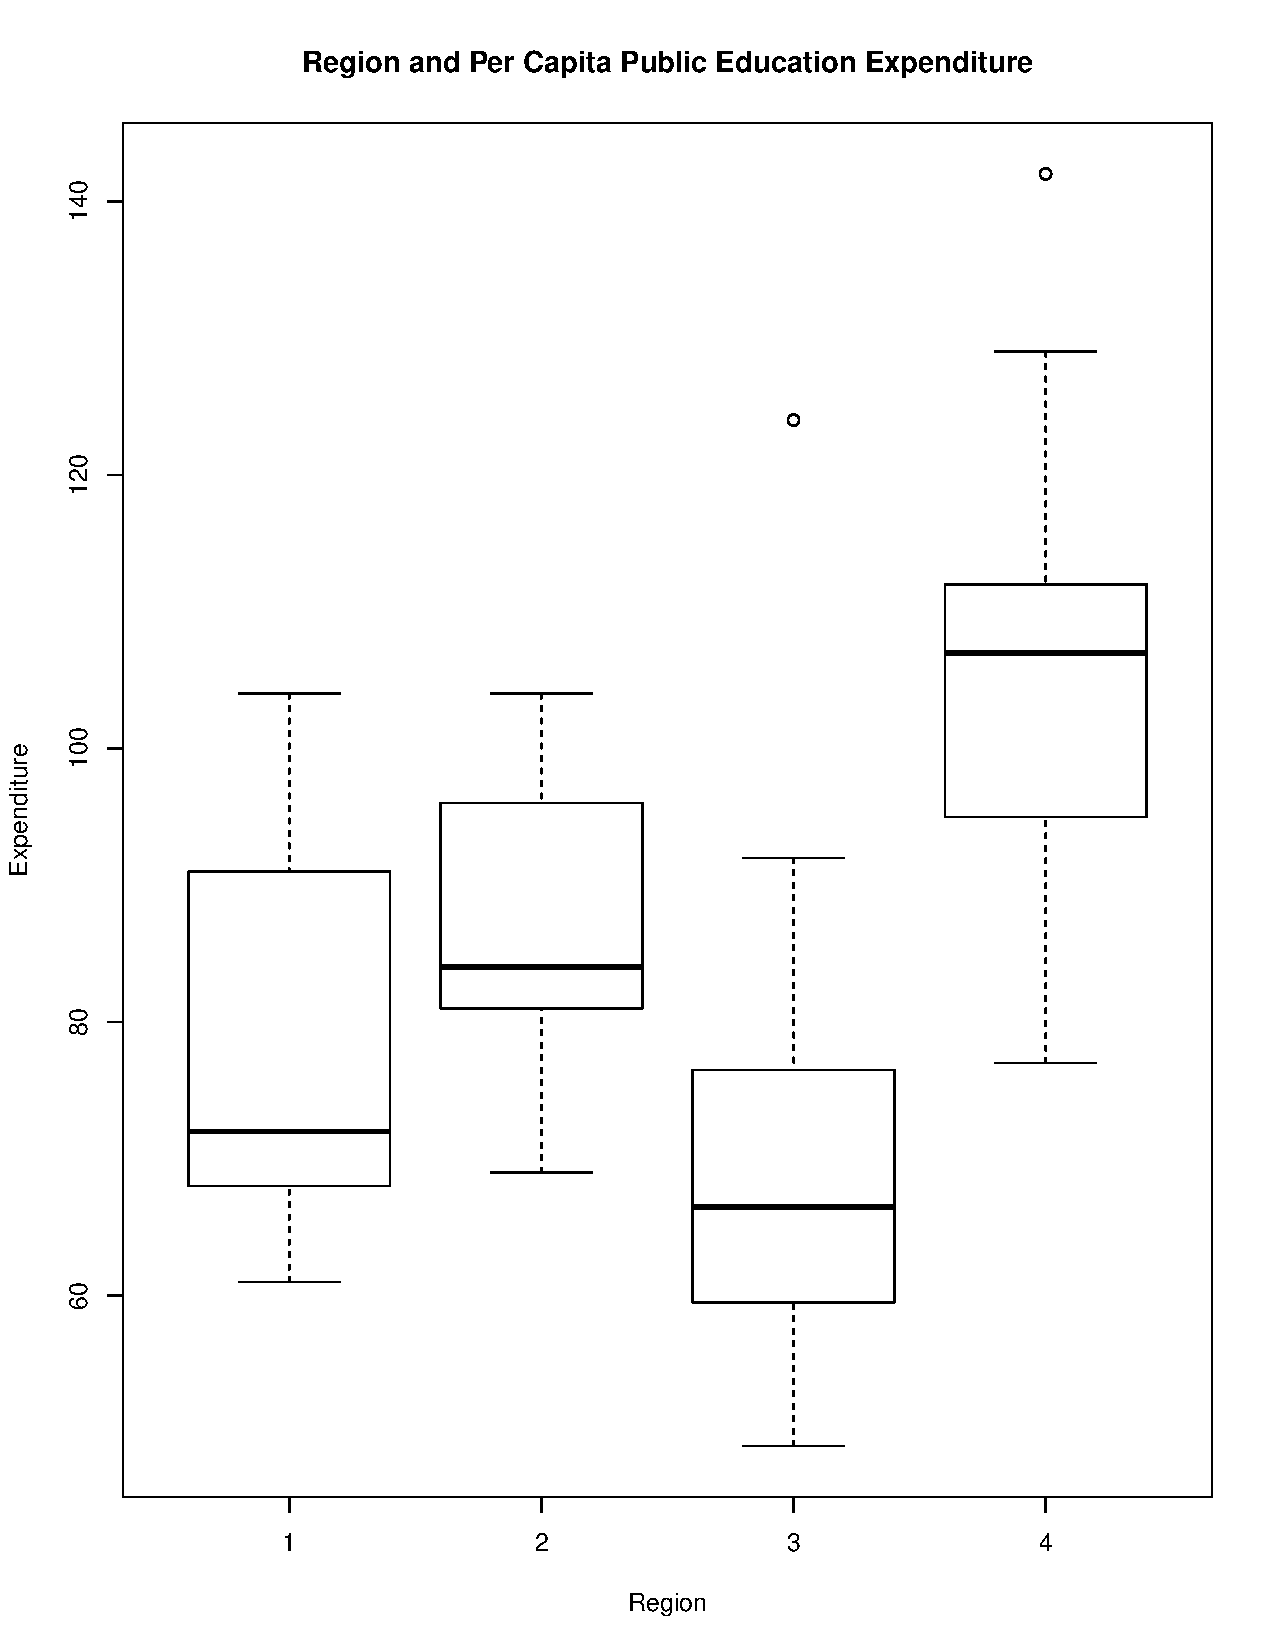
\includegraphics[width=50mm,scale=0.5]{XRegion.pdf}
\end{figure} 
\noindent Region 4 has, on average, the highest per capita expenditure on public education.
\vspace{1cm}

\item
Please plot the relationship between \emph{Y} and \emph{X1}? Describe this graph and the relationship. Reproduce the above graph including one more variable \emph{Region} and display different regions with different types of symbols and colors.
\lstinputlisting[language=R, firstline=131, lastline=131]{Sutter_ProblemSet1.R}
\begin{figure}
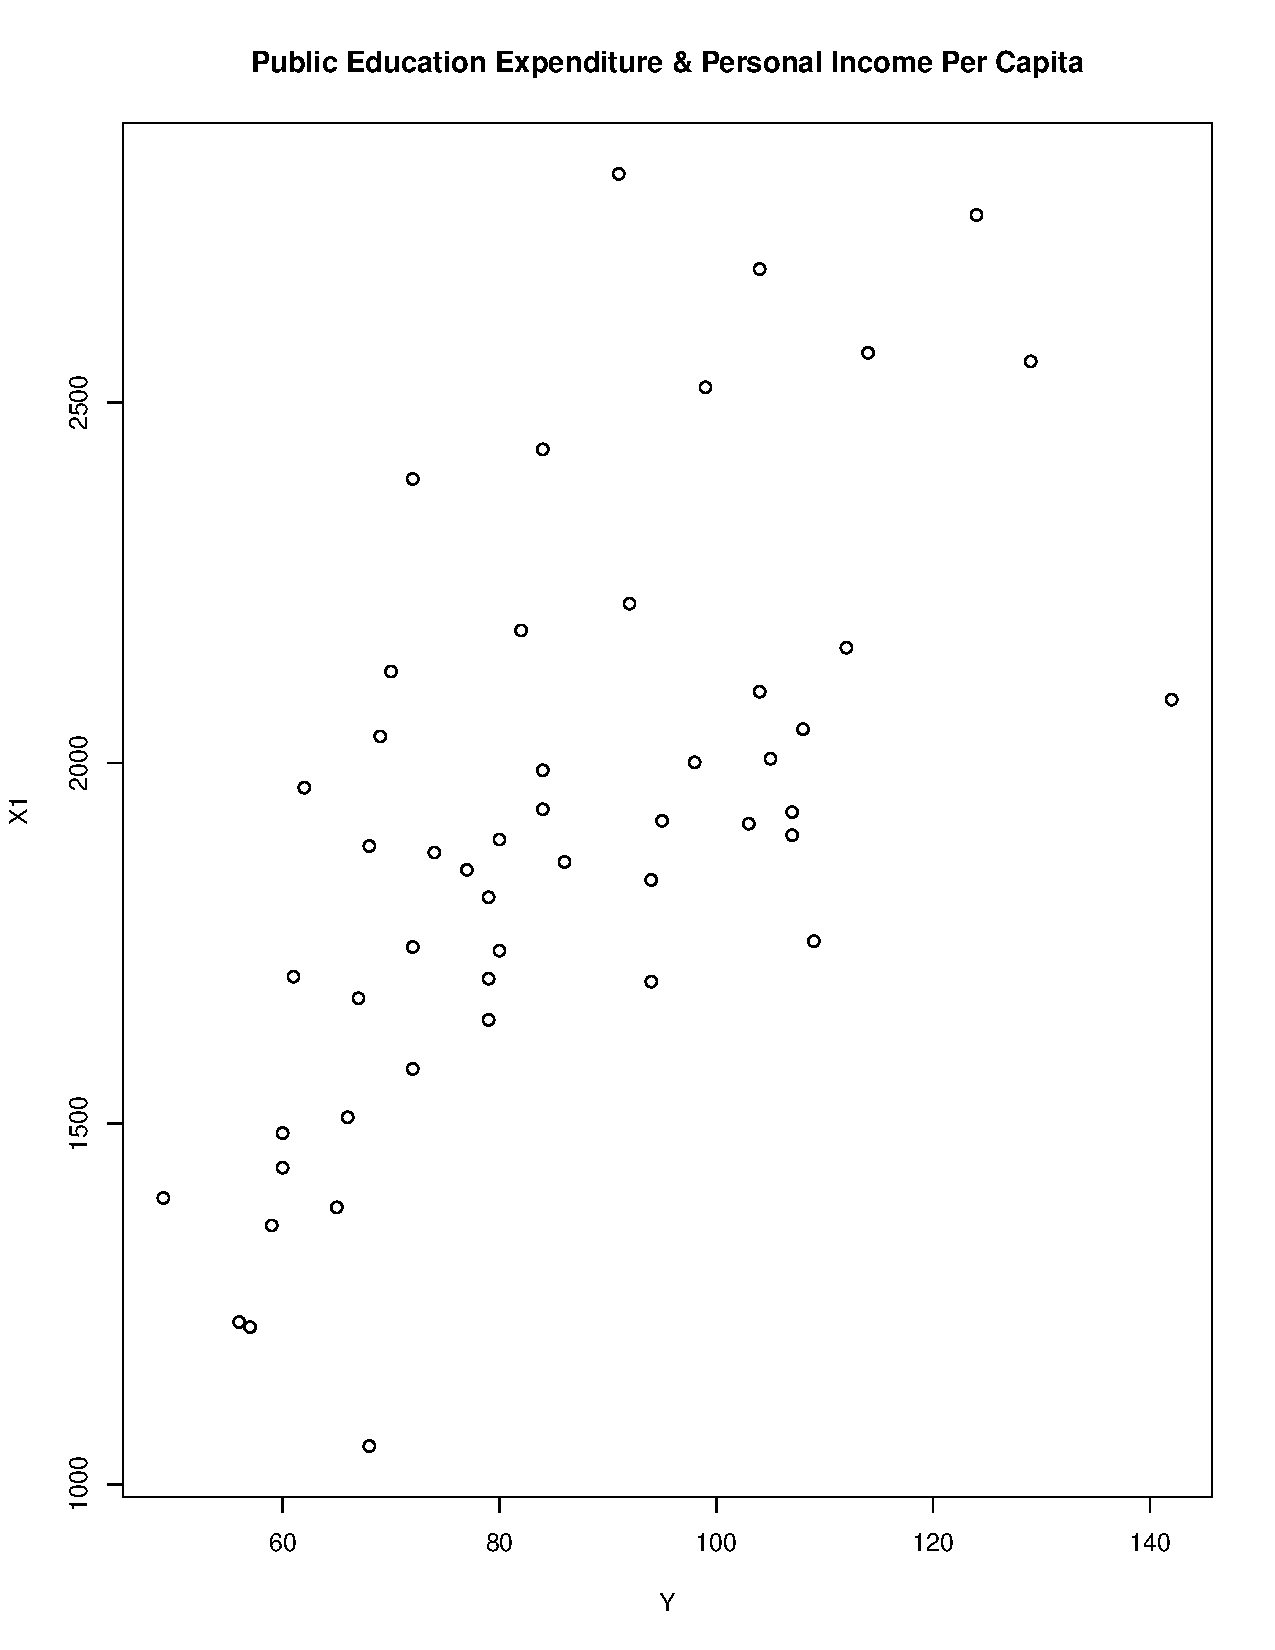
\includegraphics[width=50mm,scale=0.5]{YX1.pdf}
\end{figure} 
\noindent There is a positive association between Public Education Expenditure and Personal income per capita; as income increases, so too does spend on public education.
\lstinputlisting[language=R, firstline=135, lastline=135]{Sutter_ProblemSet1.R}
\begin{figure}
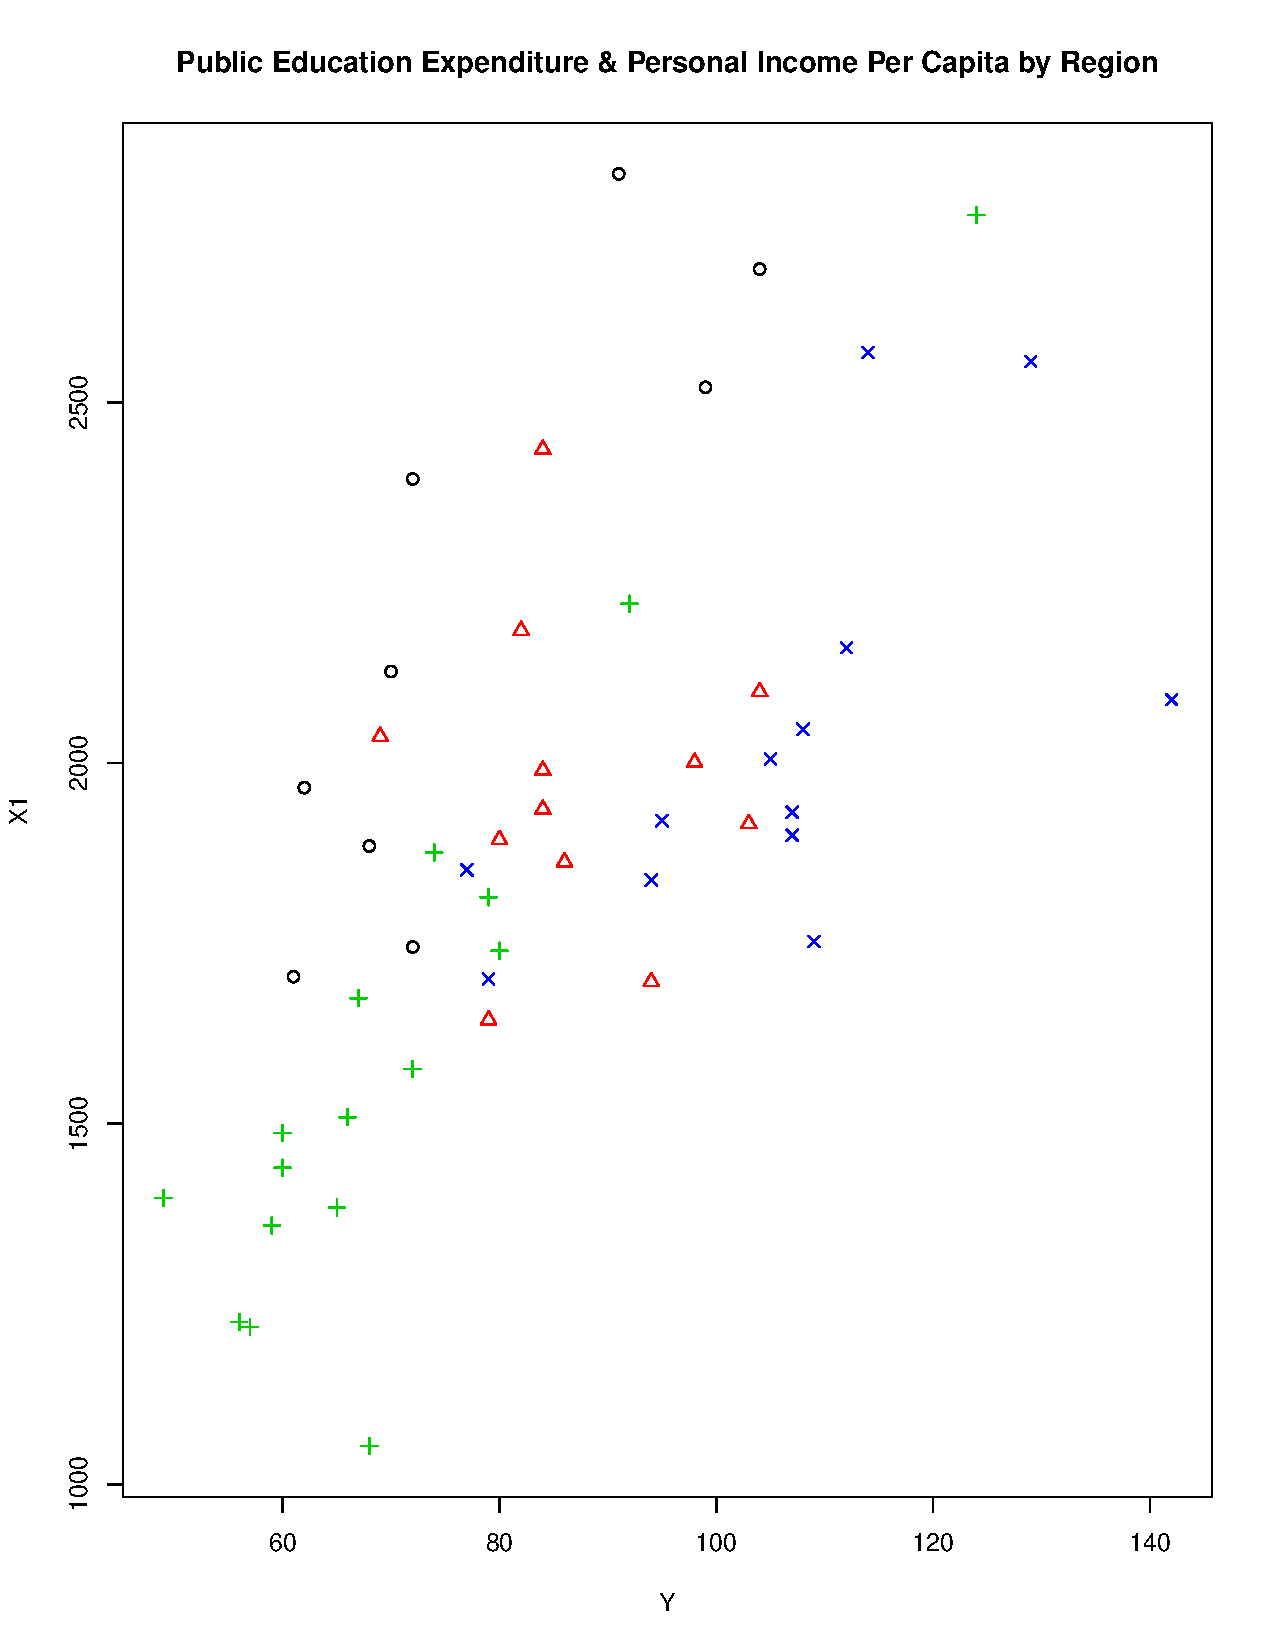
\includegraphics[width=50mm,scale=0.5]{YX1Color.pdf}
\end{figure} 

\end{itemize}

\end{document}




































